\documentclass{article}
\usepackage{graphicx}


\title{CP 8318, Assignment 3}
\author{Kody Manastyrski}
\date{01/12/2021}

\begin{document}

\maketitle

\section{Question 1}
\subsection{}

\begin{figure}
	\centering
	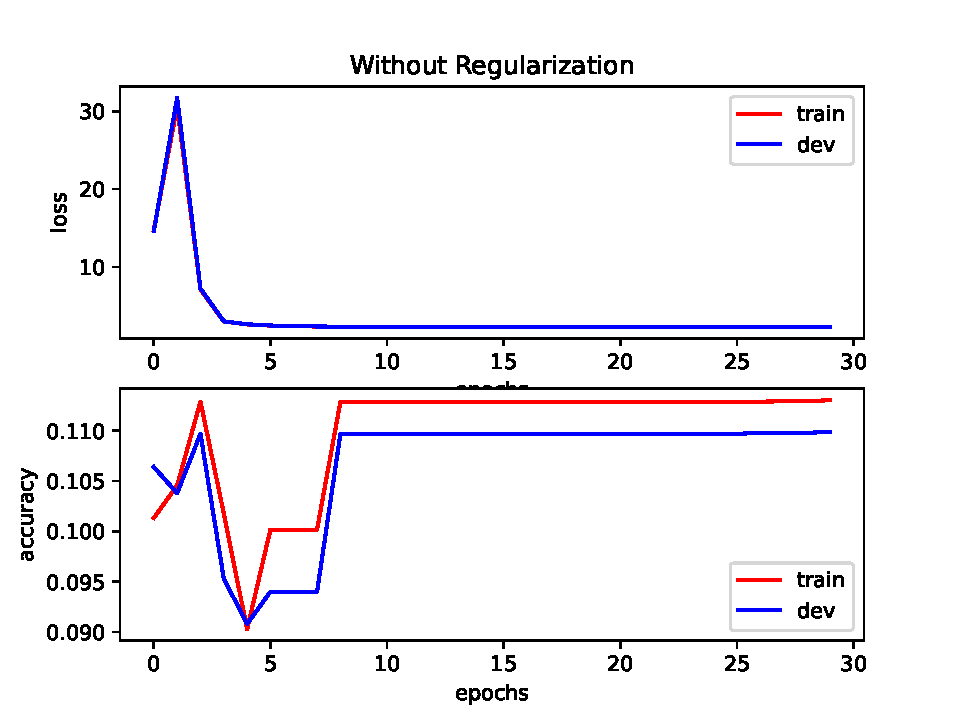
\includegraphics[width=\textwidth]{./mnist/baseline.pdf}
	\caption{'Baseline accuracy and loss vs epoch count'}
	\label{baseline}
\end{figure}

\subsection{}

\begin{figure}
	\centering
	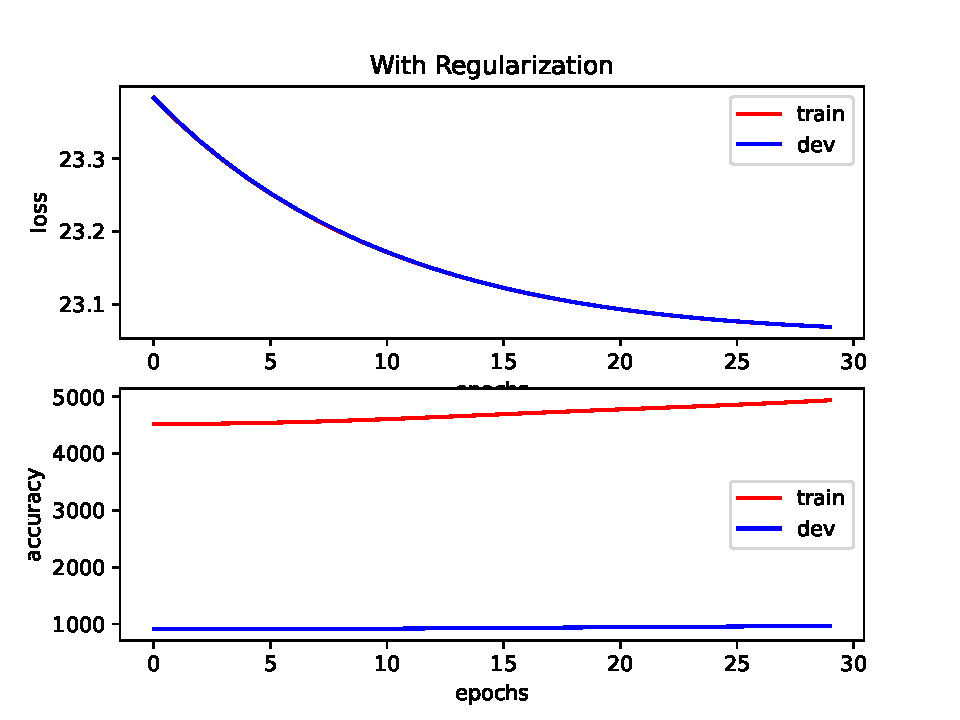
\includegraphics[width=\textwidth]{./mnist/regularized.pdf}
	\caption{'Regularized accuracy and loss vs epoch count'}
	\label{regularized}
\end{figure}

The plot of the regularized model shows a smoother descent, with significantly less amiplitude to the spikes in loss/accuracy. The regularized data, however, does not give a greater accuracy for the results, instead decresaing the accuracy. I am unsure of why this is.

\subsection{}

The accuracy remained the same between training and testing. It is still unclear as to why the regularization decreased the accuracy. Unfortunately I have run out of time, and since this assignment has been my life (to the exclusion of other work which will cost me a class if I'm not lucky) since it was released I will be submitting what I have and washing my hands of it. My the spirit of Mariah Carey's awful seasonal song embrace this assingment with all the malice it brings to retail workers. 

\end{document}




